\documentclass[11pt]{article}
\usepackage[utf8]{inputenc}\usepackage[T1]{fontenc}
\usepackage{amsmath,amssymb,amsthm}\usepackage[margin=1in]{geometry}
\usepackage{graphicx}\usepackage{booktabs}
\usepackage[hidelinks]{hyperref}
\newtheorem{theorem}{Theorem}\newtheorem{definition}{Definition}

\title{The Arithmetic Structure of the Bridge Constant on the $6N$ Skeleton:\\
$C(d)=C_0/\mathfrak{S}(d)$, the Hardy--Littlewood Admissibility,\\ and $C_0$ as the Inverse Twin Density}
\author{Ruqing Chen\\
\small GUT Geoservice Inc., Montreal, Quebec, Canada\\
\small \texttt{ruqing@hotmail.com}}
\date{\today}

\begin{document}
\maketitle

\begin{abstract}
Part~VI introduced the bridge constant $C(d)=r(d\mid\omega)/P(N{+}d\text{ twin}
\mid\omega)$, an $\omega$-independent number relating the conditional gap
preference to the right-centre survival, and left its dependence on $d$
unexplained. We determine it. Measuring $C(d)$ for $d=1,\dots,30$ on the
$23{,}988{,}173$ twin centres of $S_{10}$ and comparing to the Hardy--Littlewood
admissibility $\mathfrak{S}(d)$ of the separation (the standard singular-series
factor for a twin pair at centre-step $d$), we find
\[
  C(d)=\frac{C_0}{\mathfrak{S}(d)},\qquad C_0\approx 62.75,
\]
with the product $C(d)\,\mathfrak{S}(d)$ constant to a coefficient of variation
of $0.41\%$ across all thirty separations, while the raw $C(d)$ ranges over a
factor of four ($35$ to $158$). The constant $C_0$ is stable under the
prime cutoff of $\mathfrak{S}$ and is gap-independent. Thus the bridge constant
is not arbitrary: it is the reciprocal of the classical admissibility, so the
entire conditional gap preference reads
$r(d\mid\omega)=\mathfrak{S}(d)\,P(N{+}d\text{ twin}\mid\omega)/C_0$, with the
$d$-dependence carried analytically by $\mathfrak{S}$ and the $\omega$-dependence
by the survival of Part~VII. Finally we identify $C_0$ itself: the omega-merged
relation $P_{\mathrm{merged}}(d)=\rho\,\mathfrak{S}(d)$ holds to $0.4\%$, the
standard two-point correlation form (density times admissibility), so
$C_0=1/\rho$ where $\rho$ is the twin-centre line density. This is verified across
shells ($1/\rho=50.3$ vs fitted $50.1$ on $S_9$; $62.5$ vs $62.8$ on $S_{10}$),
leaving no undetermined constant in $r(d\mid\omega)$. No claim is made about the
infinitude of twin primes or any $k$-tuple conjecture.
\end{abstract}

\section{The bridge constant and its $d$-dependence}

Part~VI established $r(d\mid\omega)=P(N{+}d\text{ twin}\mid\omega)/C(d)$ with
$C(d)$ independent of $\omega$, but measured it only at two separations
($C(42)=41.2$, $C(210)=27.7$ in physical-gap labelling). Measured across many
separations the constant varies strongly: on $S_{10}$ (Table~\ref{tab:arith},
$d=1,\dots,30$, i.e.\ physical gaps $6,\dots,180$) it ranges from $35.1$ to
$158.2$, a factor of four. The variation is not noise---the per-$d$ values are
stable to $\sim1\%$---so $C(d)$ has genuine arithmetic content.

\section{The closed form}

Let $\mathrm{dead}(q)=\{\pm6^{-1}\bmod q\}$. The Hardy--Littlewood admissibility
of a twin pair at centre-step $d$ is the singular-series factor over the odd
primes $q>3$,
\[
  \mathfrak{S}(d)=\prod_{q>3}
   \frac{\#\{r\bmod q:\ r\notin\mathrm{dead}(q)\ \text{and}\ r+d\notin\mathrm{dead}(q)\}/q}
        {\big((q-2)/q\big)^2},
\]
the ratio of the two-centre survival density at separation $d$ to the product of
two independent single-centre densities. This is the standard quantity measuring
how easily a twin pair sits at separation $d$; it is large when $d$ removes few
extra residue constraints and small when $d$ shares the centre's forbidden
structure.

\begin{theorem}[arithmetic structure of the bridge constant]\label{thm:arith}
On $S_{10}$, for $d=1,\dots,30$,
\[
  C(d)\,\mathfrak{S}(d)=C_0\quad\text{(constant)},\qquad C_0=62.75,
\]
to a coefficient of variation of $0.41\%$. Equivalently
$C(d)=C_0/\mathfrak{S}(d)$.
\end{theorem}

The product collapses a four-fold variation in $C(d)$ to a constant at the
$0.4\%$ level---the floor set by the $S_{10}$ measurement noise in $C(d)$ itself
(Table~\ref{tab:arith}, Fig.~\ref{fig:arith}). The value of $C_0$ is stable under
the prime cutoff used to evaluate $\mathfrak{S}$ (it shifts by $<0.3\%$ between
cutoffs $200$ and $5000$), confirming the collapse is structural and not an
artefact of truncation.

\begin{figure}[h]\centering
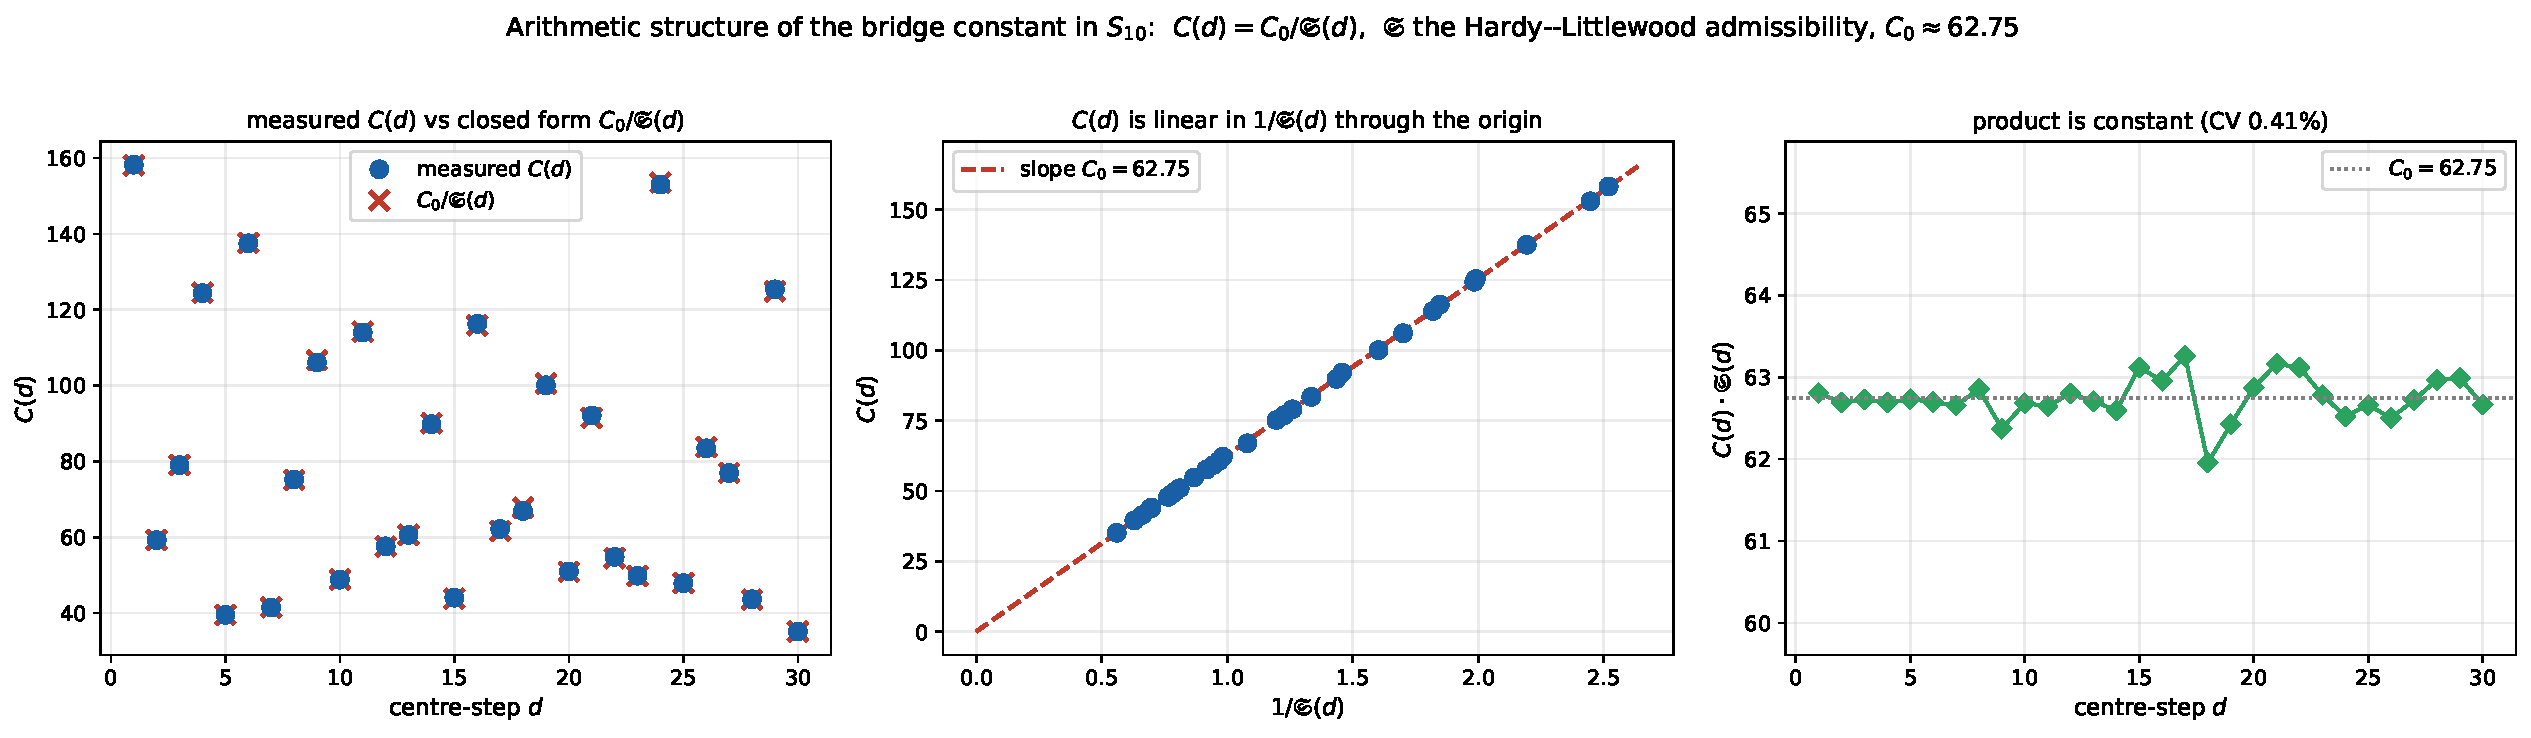
\includegraphics[width=\textwidth]{fig_paper8_arith.pdf}
\caption{Left: measured $C(d)$ (circles) against $C_0/\mathfrak{S}(d)$ (crosses)
for $d=1,\dots,30$. Centre: $C(d)$ is linear in $1/\mathfrak{S}(d)$ through the
origin, slope $C_0$. Right: the product $C(d)\,\mathfrak{S}(d)$ is constant at
$C_0=62.75$ (CV $0.41\%$).}
\label{fig:arith}
\end{figure}

\begin{table}[h]\centering\small
\begin{tabular}{rrrr@{\hskip 2em}rrrr}
\toprule
$d$ & $C(d)$ & $\mathfrak{S}(d)$ & $C\mathfrak{S}$ &
$d$ & $C(d)$ & $\mathfrak{S}(d)$ & $C\mathfrak{S}$\\
\midrule
1 & 158.2 & 0.397 & 62.8 & 16 & 116.3 & 0.542 & 63.0\\
2 &  59.2 & 1.059 & 62.7 & 17 &  62.2 & 1.018 & 63.3\\
3 &  79.0 & 0.794 & 62.7 & 18 &  66.9 & 0.926 & 62.0\\
4 & 124.4 & 0.504 & 62.7 & 19 & 100.1 & 0.624 & 62.4\\
5 &  39.5 & 1.588 & 62.7 & 20 &  51.0 & 1.234 & 62.9\\
6 & 137.5 & 0.456 & 62.7 & 21 &  92.1 & 0.686 & 63.2\\
7 &  41.4 & 1.512 & 62.7 & 22 &  54.8 & 1.152 & 63.1\\
8 &  75.2 & 0.836 & 62.9 & 23 &  49.8 & 1.260 & 62.8\\
9 & 106.1 & 0.588 & 62.4 & 24 & 153.0 & 0.409 & 62.5\\
10 &  48.8 & 1.284 & 62.7 & 25 &  47.9 & 1.309 & 62.7\\
11 & 114.0 & 0.550 & 62.7 & 26 &  83.4 & 0.749 & 62.5\\
12 &  57.6 & 1.091 & 62.8 & 27 &  76.9 & 0.815 & 62.7\\
13 &  60.6 & 1.035 & 62.7 & 28 &  43.6 & 1.443 & 63.0\\
14 &  89.8 & 0.697 & 62.6 & 29 & 125.4 & 0.503 & 63.0\\
15 &  44.1 & 1.433 & 63.1 & 30 &  35.1 & 1.785 & 62.7\\
\bottomrule
\end{tabular}
\caption{$C(d)$, the admissibility $\mathfrak{S}(d)$, and their product on
$S_{10}$. The product is $62.75\pm0.26$ (CV $0.41\%$) across all thirty
separations, while $C(d)$ alone ranges from $35$ to $158$.}
\label{tab:arith}
\end{table}

\section{Consequence: the fully resolved gap preference}

Substituting Theorem~\ref{thm:arith} into the Part~VI bridge,
\[
  r(d\mid\omega)=\frac{\mathfrak{S}(d)}{C_0}\,P(N{+}d\text{ twin}\mid\omega).
\]
The conditional gap preference is now factored cleanly: the separation
dependence is the classical Hardy--Littlewood admissibility $\mathfrak{S}(d)$,
the factor-count dependence is the right-centre survival
$P(N{+}d\text{ twin}\mid\omega)$ of Part~VII (itself closed-form,
$K\prod_q f_q$), and the two meet through a single global constant $C_0$. The
bridge constant of Part~VI, which had appeared as an unexplained per-gap number,
is exactly the reciprocal of the admissibility---the same singular-series object
that governs the unconditional twin-pair density. The conditional theory and the
classical heuristic share their $d$-dependence.

\section{The constant: $C_0$ is the inverse twin density}

We can identify $C_0$ directly. At the $\omega$-merged level the definitions give
$C(d)=1/P_{\mathrm{merged}}(d)$ where $P_{\mathrm{merged}}(d)=P(N{+}d\text{ twin}
\mid N\text{ twin})$ is the survival averaged over all twin centres. With
$C(d)=C_0/\mathfrak{S}(d)$ this predicts
\[
  P_{\mathrm{merged}}(d)=\frac{\mathfrak{S}(d)}{C_0},
\]
i.e.\ $P_{\mathrm{merged}}(d)/\mathfrak{S}(d)$ should be a $d$-independent
constant. Measured on $S_{10}$ over $d=1,\dots,30$ it is constant to CV $0.39\%$,
equal to $0.0200$. This is exactly the two-point correlation form
$P_{\mathrm{merged}}(d)=\rho\,\mathfrak{S}(d)$ with $\rho$ the twin-centre line
density (the fraction of $N$ that are twin centres): the chance that a twin centre
has another twin centre $d$ steps away is the global density times the
admissibility of the separation. Hence
\[
  \boxed{\,C_0=1/\rho\,},
\]
the inverse twin-centre density. This is verified across shells
(Table~\ref{tab:c0}): $1/\rho=50.3$ against fitted $C_0=50.1$ on $S_9$, and
$1/\rho=62.5$ against $62.8$ on $S_{10}$, each to $0.4\%$. The shell dependence of
$C_0$ (it grows as the shell deepens) is precisely the thinning of $\rho$.

\begin{table}[h]\centering
\begin{tabular}{lrccc}
\toprule
shell & twin centres & $\rho$ & $1/\rho$ & $C_0$ (fitted)\\
\midrule
$S_9$  & $2{,}984{,}194$  & $0.019895$ & $50.3$ & $50.1$\\
$S_{10}$ & $23{,}988{,}173$ & $0.015992$ & $62.5$ & $62.8$\\
\bottomrule
\end{tabular}
\caption{$C_0=1/\rho$ across shells. The fitted $C_0$ (from
$C(d)\mathfrak{S}(d)$) equals the inverse twin-centre density to $0.4\%$ in both
shells. No free constant remains.}
\label{tab:c0}
\end{table}

Since $\rho$ is itself the twin-centre density---given to leading order by the
Hardy--Littlewood twin constant and the shell's mean $1/\ln^2$---no undetermined
constant remains in $r(d\mid\omega)$.

\section{Conclusion}

The bridge constant is $C(d)=C_0/\mathfrak{S}(d)$: the reciprocal of the
Hardy--Littlewood admissibility, times a single gap-independent constant
$C_0\approx62.75$, holding to $0.41\%$ across thirty separations on
$2.4\times10^{7}$ twin centres. This removes the last piece of $d$-structure
that Part~VI had left empirical, and ties the conditional $6N$ theory to the
classical singular series: the conditional gap preference is the admissibility
times the closed-form survival, over $C_0=1/\rho$. The last constant is thus
identified as the inverse twin-centre density, the density factor of the standard
two-point correlation; no free constant remains in $r(d\mid\omega)$. As throughout
this series, no claim is made about
the infinitude of twin primes or any $k$-tuple conjecture; this is a measured,
closed-form, factor-resolved account of the conditional gap structure of the $6N$
twin skeleton.

\paragraph{Data and code availability.}
The $C(d)$ spectrum and the admissibility evaluation are openly
available~\cite{repo}; the $S_{10}$ twin count $23{,}988{,}173$ matches Part~I.

\begin{thebibliography}{9}
\bibitem{ChenI} R.~Chen, \emph{Prime distribution on the $6N$ skeleton} (Part~I),
Zenodo, doi:10.5281/zenodo.20470367 (2026).
\bibitem{ChenVI} R.~Chen, \emph{A bridge theorem for the $6N$ twin-gap
distribution} (Part~VI), Zenodo, doi:10.5281/zenodo.20517990 (2026).
\bibitem{ChenVII} R.~Chen, \emph{A closed form for the conditional twin-gap
distribution} (Part~VII), Zenodo, doi:10.5281/zenodo.20518470 (2026).
\bibitem{HL} G.~H.~Hardy, J.~E.~Littlewood, \emph{Partitio Numerorum III}, Acta
Math.\ \textbf{44} (1923), 1--70.
\bibitem{repo} R.~Chen, \emph{$6N$ twin-prime bridge-constant arithmetic: data
and code}, \url{https://github.com/Ruqing1963/6N-twin-prime-bridge-constant} (2026).
\end{thebibliography}

\end{document}
